\section{Whitney Music Box}
This mesmerizing applet is inspired by the animations of John Whitney (1917-1995), a filmmaker that explored and experimented with animation techniques governed by mathematical and mechanical rules, before the digital era. In the 1950s, Whitney experimented with pendulums, gears, mechanical artifacts, and early analog computers combined with cameras to produce short films of lines and dots of light, being a pioneer of video as a plastic form of abstract art. In the 1960s he embraced digital computers and devoted his career to computer graphics art, with shorts and films as Permutations (1968), Arabesque (1976), or Moon Drum (1991).

In 1980, Whitney published the book Digital Harmony, where he describes his experiments on visualizing music with computer graphics. In particular, he explains what he called ``incremental drift'', a kind of algorithm to set the position of particles, where each particle is ``drifted'' from the previous one by a simple rule; a kind of differential rule that by integration gives rise to a global behavior that was originally unexpected. Whitney gave in his book an example of this spiral incremental drift. 

In 2006, the programmer and Disney animator Jim Bumgardner took Whitney's ideas and created an interactive applet adding synchronized sound to Whitney's spirals. Bumgardner coined the term ``Whitney's music box'' and the applet has become popular on the Internet since.

\begin{figure}[h]
\centering
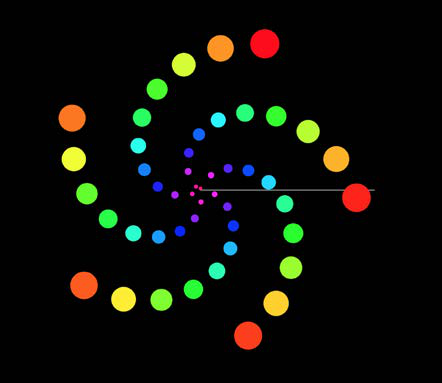
\includegraphics[width=0.5\textwidth]{Whitney_1}
\end{figure}

Mathematically the applet can be described fairly easily. Each point moves along a concentric circle, and moves at an angular speed proportional to its radius. Or said in other words: every time the innermost dot goes once around the circle, the next one goes twice, the next one goes three times, and so forth. 

The overall reference for rotation speed is given by the controlling wheel/knob. Each point plays a particular tone (assigned in the chromatic scale) when the point crosses the horizontal line. This rotations produce changing spiral patterns and chords when several tones play at once. The speed of rotation imposes a rhythmic cadence of tones that reflect the geometry of the pattern, evoking the consonance and dissonance of the notes in the scale.

This music box enables to visualize harmonic resonance and musical harmony in a pleasant way. Playful and challenging in the same time, you might find it hard to predict what will the sound and patterns resemble. It is a tool for admiration and a bit of self-hypnotic recreation.



\begin{sectcredits}
\item[Author of the exhibit:] Eric Londaits (IMAGINARY). Inspired by Jürgen Richter-Gebert's implementation.

\item[Text:] Eric Londaits and Daniel Ramos (IMAGINARY).

\item[References:] \strut
\noindent \begin{itemize}[leftmargin=*]
\item \url{https://krazydad.com/blog/2006/04/23/visual-harmony}

\item \url{https://boingboing.net/2016/04/11/john-whitney-music-box-a-psyc.html}

\item \url{https://jbum.com/papers/whitney_paper.pdf}

\item John Whitney. \emph{Digital Harmony: On the Complementarity of Music and Visual Art}. Byte Books / McGraw-Hill (1980). \\
\url{https://archive.org/details/DigitalHarmony_201611}

\end{itemize}
\end{sectcredits}
